\documentclass[aspectratio=169]{beamer}

% --------------------------------------------------
% PACOTES
% --------------------------------------------------

\usepackage[utf8]{inputenc}
\usepackage[T1]{fontenc}
\usepackage[brazil]{babel}

\usepackage{amsmath}
\usepackage{amssymb}
\usepackage{graphicx}
\usepackage{booktabs}

\usepackage{lmodern}
% --------------------------------------------------
% TEMA
% --------------------------------------------------

\usetheme{metropolis}

\setbeamertemplate{footline}{}

% --------------------------------------------------
% INFORMAÇÕES DA APRESENTAÇÃO
% --------------------------------------------------

\title{Seismic Blind Deconvolution Based on Self-Supervised \\Machine Learning (SSL-BD)}
\subtitle{Applied Sciences, 2024 - mdpi.com}

\author{Xia Yin, Wenhao Xu, Zhifang Yang, Bangyu Wu}

\institute{
    Métodos Avançados de Inteligência Artificial para Processamento de Dados Sísmicos \\
    COPPE - UFRJ
}

% --------------------------------------------------
% DOCUMENTO
% --------------------------------------------------

\begin{document}

% --------------------------------------------------
% SLIDE DE TÍTULO
% --------------------------------------------------

\begin{frame}
    \titlepage
\end{frame}

% --------------------------------------------------
% SUMÁRIO
% --------------------------------------------------

\begin{frame}{Sumário}
    \tableofcontents
\end{frame}

% --------------------------------------------------
% CONTEÚDO
% --------------------------------------------------

\section{Problema}
\begin{frame}{Problema}
    A ideia básica da deconvolução sísmica é:
    \begin{equation}
        y = w * r
    \end{equation}
    onde:
    \begin{itemize}
        \item \(y\): dado sísmico observado;
        \item \(w\): wavelet sísmica;
        \item \(r\): refletividade;
        \item \(*\): convolução
    \end{itemize}
    Blind deconvolution é um problema mal-posto e subdeterminado 
    em que $w$ e $r$ são desconhecidos
\end{frame}
\begin{frame}{Por que é um problema difícil?}
    Supondo que a verdadeira refletividade seja $r = [0,1,0,-0.5,0]$ 
    e a wavelet seja $w = [0.5,1,0.5]$;

    Dado que convolução produz $y = w * r$, em vez de vermos os dois picos de 
    refletividade diretamente, observamos versões deles "espalhadas" pela wavelet.

    Mas como saber se uma determinada estrutura em \(y\) veio da wavelet ou da 
    refletividade?

    Por exemplo, talvez uma wavelet mais estreita combinada com uma refletividade 
    mais larga produza praticamente o mesmo y.
\end{frame}
\begin{frame}{Métodos existentes}
    O artigo separa os métodos existentes em três grupos:
    \begin{enumerate}
        \item métodos clássicos;
        \item machine learning supervisionado;
        \item self-supervised learning.
    \end{enumerate}
    O problema dos métodos supervisionados é que precisamos de labels de refletividade.

    O self-supervised learning tenta contornar isso. O modelo SSL-D usa o próprio modelo 
    físico de convolução dentro da função de perda, mas precisa conhecer a wavelet.

    A novidade do SSL-BD é trabalhar com wavelet desconhecida.
\end{frame}
\section{BBL-BD}
\begin{frame}{BBL-BD}
    A ideia do BBL-BD consiste em usar o dado observado para estimar o wavelet e a 
    refletividade usando duas redes neurais combinadas
    \begin{figure}
        \centering
        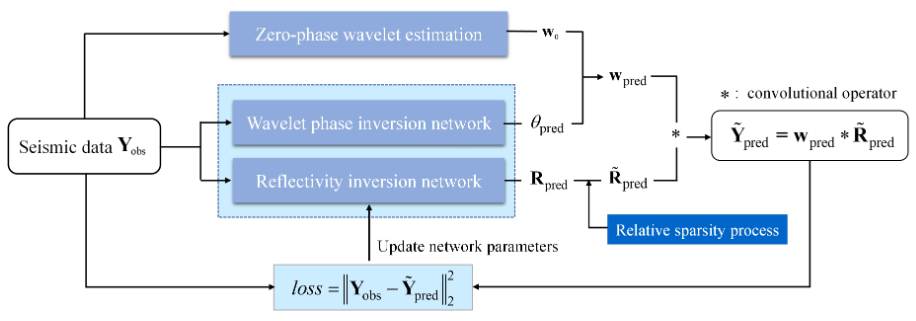
\includegraphics[width=1\linewidth]{slides/imagens/ssl-bd.png}
    \end{figure}
\end{frame}
\section{Arquitetura}
\subsection{Etapa 1}
\begin{frame}{Etapa 1}
    O método não começa a rede com uma wavelet completamente aleatória.

    Ele tenta obter uma estimativa inicial da wavelet a partir do próprio dado.
    
    Passos:
    \begin{enumerate}
        \item Cálculo da média dos traces $\bar{y} = \frac{1}{N_{traces}} \sum_{i}y_i$
        \item Cálculo da $FFT(\bar{y})$ e espectro de amplitude $|FFT(\bar{y})|$
        \item Suavização do espectro de amplitude com um polinômio cúbico local de 7 pontos (filtro de Savitzky-Golay)
        \item Aplicação da IFFT ao espectro suavizado
    \end{enumerate}

    A wavelet inicial ($w_0$) é calculada como $IFFT(smooth(|FFT(\bar{y})|))$

    %$w_0$ é uma estimativa de wavelet de fase zero que fornece essencialmente 
    %a informação de amplitude da wavelet. A rede neural aprende principalmente 
    %a fase da wavelet ($\theta$).

\end{frame}
\subsection{Etapa 2}
\begin{frame}{Etapa 2}
    A próxima estapa estima a fase $\theta$
    \begin{equation}
        \theta_{pred} = NN_{\theta} (Y_{obs};\phi_{\theta})
    \end{equation}
    A arquitetura possui:
    \begin{itemize}
        \item 4 camadas convolucionais;
        \item 2 fully connected layers.
    \end{itemize}
    A primeira convolução usa kernel \(29\times1\) e stride 14.

    As seguintes usam \(4\times1\) e stride 2.

    Depois ocorre flattening e duas camadas fully connected, resultando em um único valor de fase.

    O método usa a transformada de Hilbert para girar $w_0$ no domínio de fase por $\theta$
    \begin{equation}
        w_{pred} = Re[(w_0 + j Hilbert(w_0)) e^{-j\theta_{pred}}]
    \end{equation}
\end{frame}
\subsection{Etapa 3}
\begin{frame}{Etapa 3}
    A terceira estapa estima a fase $\theta$
    \begin{equation}
        \theta_{pred} = NN_{\theta} (Y_{obs};\phi_{\theta})
    \end{equation}
    A arquitetura possui:
    \begin{itemize}
        \item 4 camadas convolucionais;
        \item 2 fully connected layers.
    \end{itemize}
    A primeira convolução usa kernel \(29\times1\) e stride 14.

    As seguintes usam \(4\times1\) e stride 2.

    Depois ocorre flattening e duas camadas fully connected, culminando em um único valor de fase.
\end{frame}
\begin{frame}{Sumarização do método}
    O método emprega uma restrição de sparsity relativa, 
    em que o threshold ($\mu$) de sparsity muda durante o treinamento
    com base em $r_{epoch} = \frac{\text{época atual}}{\text{total de épocas}}$
    
    \begin{enumerate}
        \item Rede recebe $Y_{obs}$
        \item Rede produz $R_{pred}$ e $\theta_{pred}$
        \item Com $\theta_{pred}$, calcula-se $w_{pred}$
        \item Aplica-se sparsity $R_{pred} \rightarrow \bar{R}_{pred}$
        \item Faz-se a operação física $\bar{Y}_{pred} = w_{pred} * \bar{R}_{pred}$
        \item A perda é calculada como $\mathcal{L} = || Y_{obs} - \bar{Y}_{pred} ||_2^2$
    \end{enumerate}
\end{frame}

\end{document}
